
\chapter{系统架构}

\section{需求分析}

\label{requireAnalysis}

对于一个行政管理系统而言,最首要的工作是要确定需求。在进行系统架构的设计之前,我们和清华大学工会负责人讨论确定了系统的需求。

图\ref{fig:demand}展示了我们整理的工会管理系统需要实现的功能流程图。

\begin{figure}[H]
  \centering
  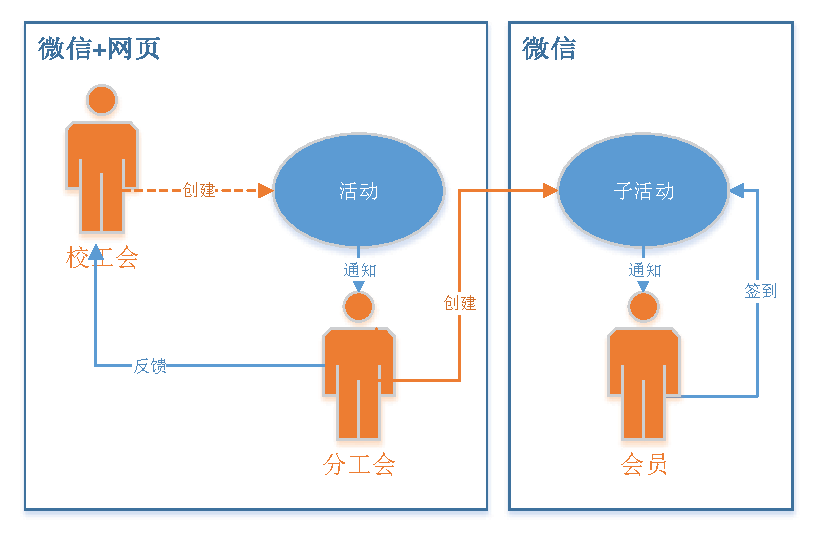
\includegraphics{demand}
  \caption{工会管理系统总体需求流程图}
  \label{fig:demand}
\end{figure}

由需求图中可以看到,整个工会行政过程分为六个主体部分:总工会发起活动,分工会反馈,授权人指定,子活动创建,子活动追踪,以及生成活动报告。通过进一步对需求进行分析可以发现,在工会的管理过程中涉及到三个角色:校工会,分工会和会员。这三种角色的具体职责如图\ref{fig:demand2}所示。

\begin{figure}[H]
  \centering
  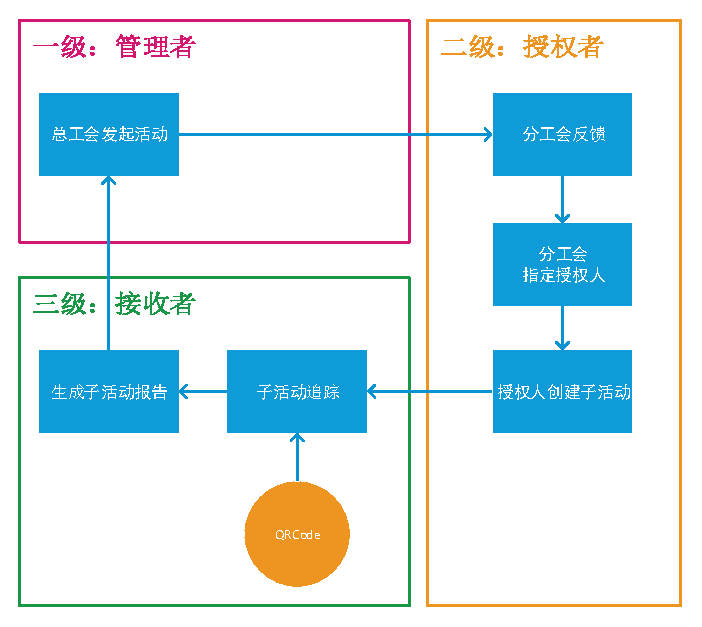
\includegraphics{demand2}
  \caption{工会行政中三种角色及其职责分析}
  \label{fig:demand2}
\end{figure}

更具体的,各个角色的职责可以描述为:

\begin{itemize}
	\item 校工会主席:负责创建一个活动,向分工会主席进行通知并接受一个活动的反馈报告信息;
	\item 分工会主席:负责接收校工会创建的活动,针对活动的要求创建对应的子活动,并将子活动的进行结果制成报告反馈回校工会;
	\item 工会会员:接收子活动推送,参加活动并参与签到。
\end{itemize}

在完成了这些需求的分析和角色的划分之后,就能够开始进行对系统架构的设计和实现工作了。

\section{B/S和C/S混合框架}

正如标题中所言,本文中的系统采用的是B/S和C/S混合系统。B/S架构使用的是浏览器/服务器结构,而C/S架构指的是客户端和服务器结构。即在使用系统的时候,一套Server需要服务两套客户前端。图\ref{fig:overallArchitecture}是一个系统的总体框架示意图,展示了B/S和C/S架构在本文中的系统中的关系。

\begin{figure}[H]
  \centering
  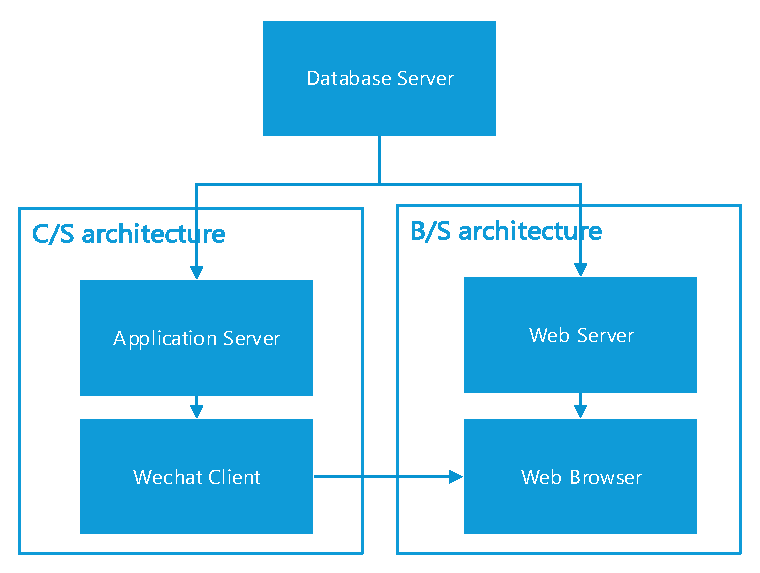
\includegraphics{overallArchitecture}
  \caption{系统的B/S和C/S混合框架}
  \label{fig:overallArchitecture}
\end{figure}

这样设计的原因是借助了桌面平台能够高效率地进行输入工作,并且输入工作对移动性的需求并不高,能够使用浏览器实现跨平台和设备无关就已经能够满足信息的录入对移动便携的需求。另一方面,对于工会活动信息的接收者来说,他们需要随时随地地接收到工会的推送活动消息。目前的浏览器并不能支持实时的消息推送。要实现这一步,需要通过一个浏览器,即本例中的微信企业号微平台,来实现这一步。

其中一个客户前端是传统B/S架构中的Brower角色,即浏览器。用浏览器代替传统的桌面计算机设备上的应用程序,使得系统能够原生地利用浏览器的跨平台特性从而实现跨平台的效果。即无论是在Windows操作系统中还是在OSX操作系统,都可以通过浏览器访问到系统的浏览器客户端,并对系统进行控制和管理。在本文中实现的系统中,甚至实现了可以在手机的浏览器上访问浏览器客户端的内容,实现了高度的兼容性。

另一方面,系统架构中的C/S架构部分则区别于传统的C/S架构。它并不是基于一个独立的移动端应用程序,而是作为微信客户端中“企业号”功能中的一个子项目微平台存在。区别于B/S架构中的浏览器成分,微信中的微平台能够提供浏览器所没有办法提供的推送功能,相当于一个小型的客户端程序。在这样一个麻雀虽小五脏俱全的微型客户端中,结合微信提供的内置浏览器和二维码扫描功能,能够实现包括查看、接收和管理活动的同时,还能进行网页浏览器无法进行的二维码签到功能。

\section{系统架构}

由于系统涉及到两个独立的前端,因此一个解决方法是参考REST架构,将前后端的设计进行分离。如图\ref{fig:architecture}是本系统架构的示意图。

\begin{figure}[H]
  \centering
  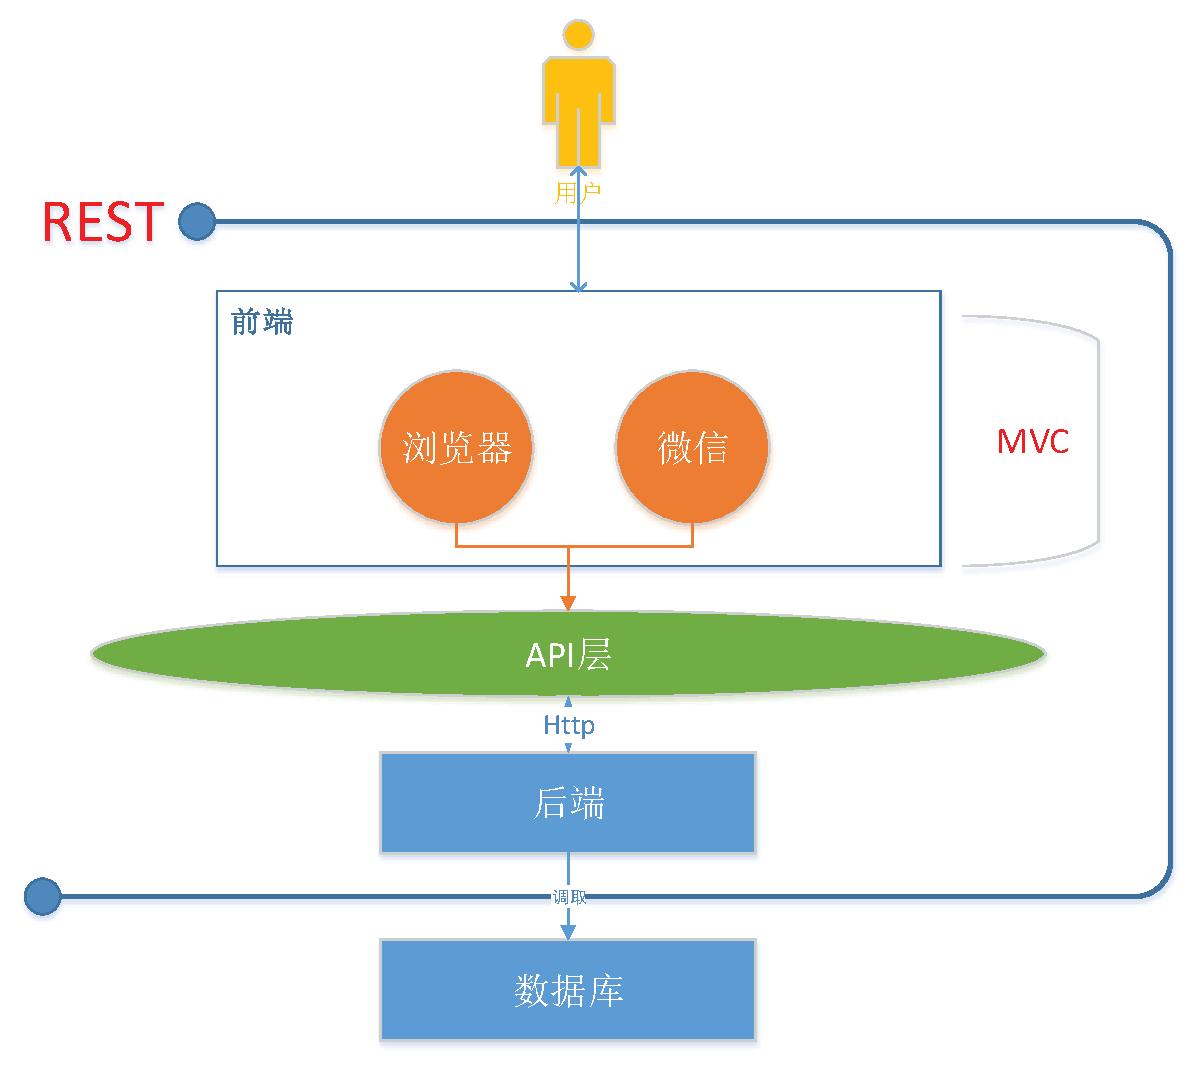
\includegraphics[width=0.8\textwidth]{architecture}
  \caption{系统架构示意图}
  \label{fig:architecture}
\end{figure}

下面将分成前端架构、后端架构和前后端通信三个部分分别对架构进行具体的描述。

\subsection{前端架构}

凭借AngularJS的强大功能,极大地简化了在前端进行网页应用程序开发的过程,并使得前端也能够拥有原来只有在后端才能够实现的MVC架构。前端架构如图\ref{fig:frontMVC}所示。

\begin{figure}[H]
  \centering
  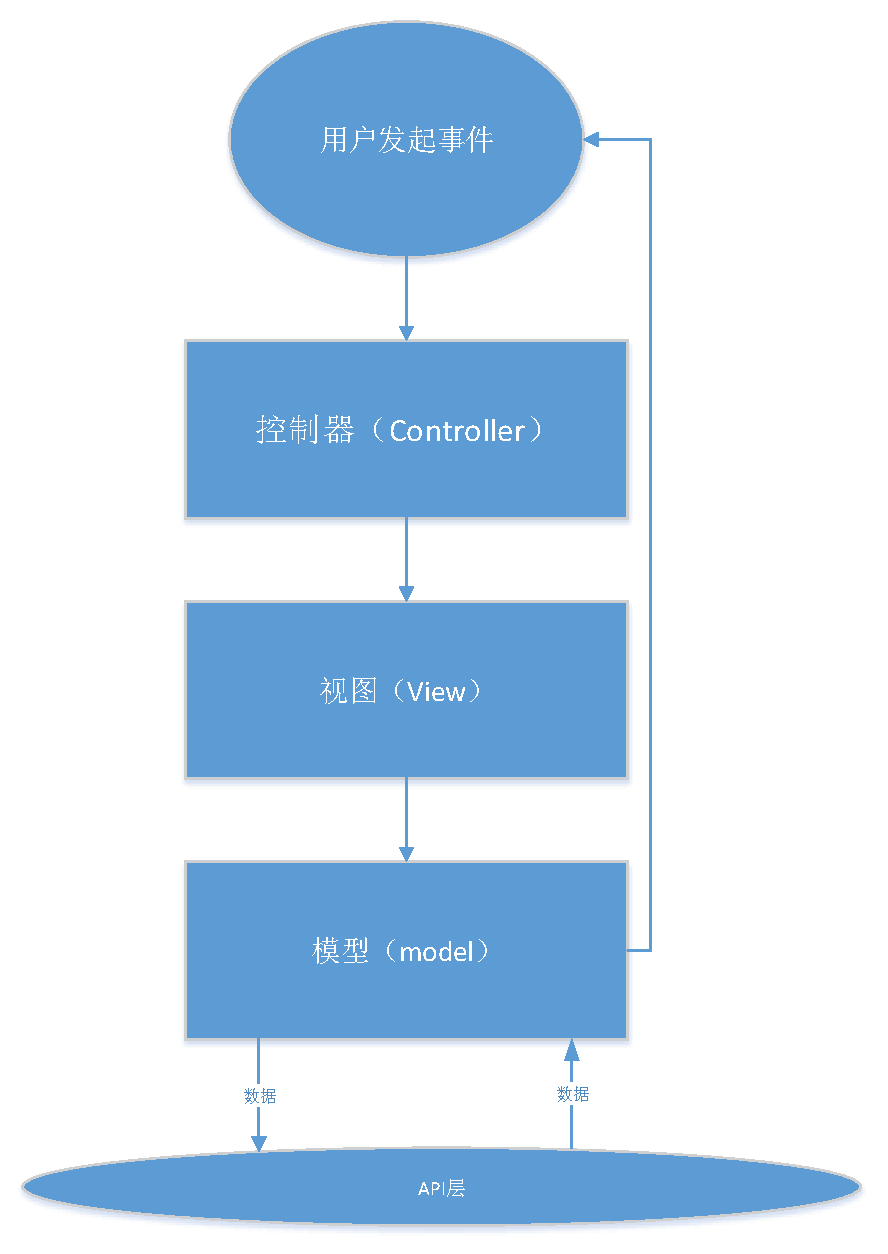
\includegraphics[width=0.5\textwidth]{frontMVC}
  \caption{前端MVC架构示意图}
  \label{fig:frontMVC}
\end{figure}

由前端的控制器接受并响应用户事件,控制视图对页面上对应的元素进行修改,并由视图访问模型元件对API进行调用的过程。由一些具有树状关系的控制器控制多个视图对不同的事件进行响应,同时控制器控制不同的模型对不同的API进行数据的调用和读取请求,使得后端能够对前端的事件作出不同的相应。

在前端使用MVC架构使得前端能够在不刷新页面的情况下,仅仅通过切换视图就可以达到展现不同页面的效果,同时保证了前端数据的去耦合。以MVC架构作为前端设计的页面,规避了Javascript长久以来受人诟病的代码凌乱问题,使得各个部分的代码各司其职,方便模块化进行维护,同时也提供了高度的可拆装性。

有关AngularJS的具体描述,将在\ref{angularJS}节进行详细展开。

\subsection{后端架构}

后端使用了JAVA Servlet作为后端服务器,以Apache Tomcat作为运行环境。由于使用了REST架构,因此后端不涉及数据的显示工作,因此主要包含了四个部分:功能类、数据模型类、Bean类和API类。四个类的具体描述如下:

\begin{itemize}
	\item 功能类:提供与HTTP请求数据无关的功能方法;
	\item 数据模型类:与数据库进行直接通讯的类,将各种对数据库的操作进行封装,使得API类能够通过调用数据模型类的方法可以间接方便地对数据库进行处理;
	\item Bean类:对数据表中的数据格式进行封装,使得API类能够通过JAVA的方式对数据库中的数据进行处理;
	\item API类:唯一的接受HTTP请求并对HTTP请求进行回应的类。
\end{itemize}

更具体的,后端架构如图\ref{fig:backend}所示。

\begin{figure}[H]
  \centering
  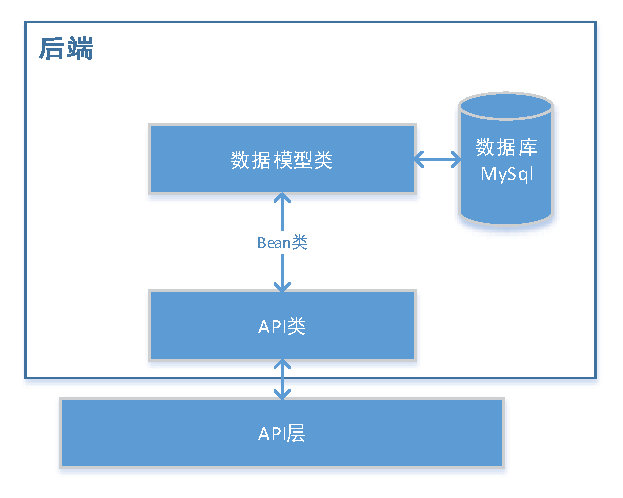
\includegraphics{backend}
  \caption{后端架构示意图}
  \label{fig:backend}
\end{figure}

通过这样的设计能够使得在设计API的过程中无需考虑对数据库的处理,而设计数据模型类的时候,也可以忽略上层对它的调用情况,实现代码的灵活拆装。

\subsection{前后端通信}

从图\ref{fig:frontMVC}和图\ref{fig:backend}中可以看到,前后端的通信是通过API层来完成的。而API层的实质是HTTP的GET和POST请求。

在REST架构中,后端不负责呈现页面,同样的前端也不负责数据的处理逻辑。前端的数据模型模块将参数打包成JSON,通过AJAX技术以HTTP GET或者POST请求发送到指定API的URL位置。此时后端的服务器中运行的Servlet会收到这个HTTP请求,并解析HTTP请求中的JSON参数进行处理,然后将结果重新打包成JSON的格式,以HTTP Response的形式返回给前端。这样一次前端对后端的调用就完成了。

更详细的对于REST架构的描述,可以参见\ref{rest}。

\section{数据库设计}

一个优秀的数据库设计可以使得服务器后端在处理相应的时候有更快的相应速度,并降低数据库的存取压力。

在本文的系统中,我们使用了MySql关系型数据库作为后端的数据提供者。MySQL是目前最流行的关系型数据库管理系统,通过灵活地使用外链索引,能够将不同的数据表之间的数据栏目进行关联。

本系统中数据库UML图如图\ref{fig:uml}所示。

\begin{figure}[H]
  \centering
  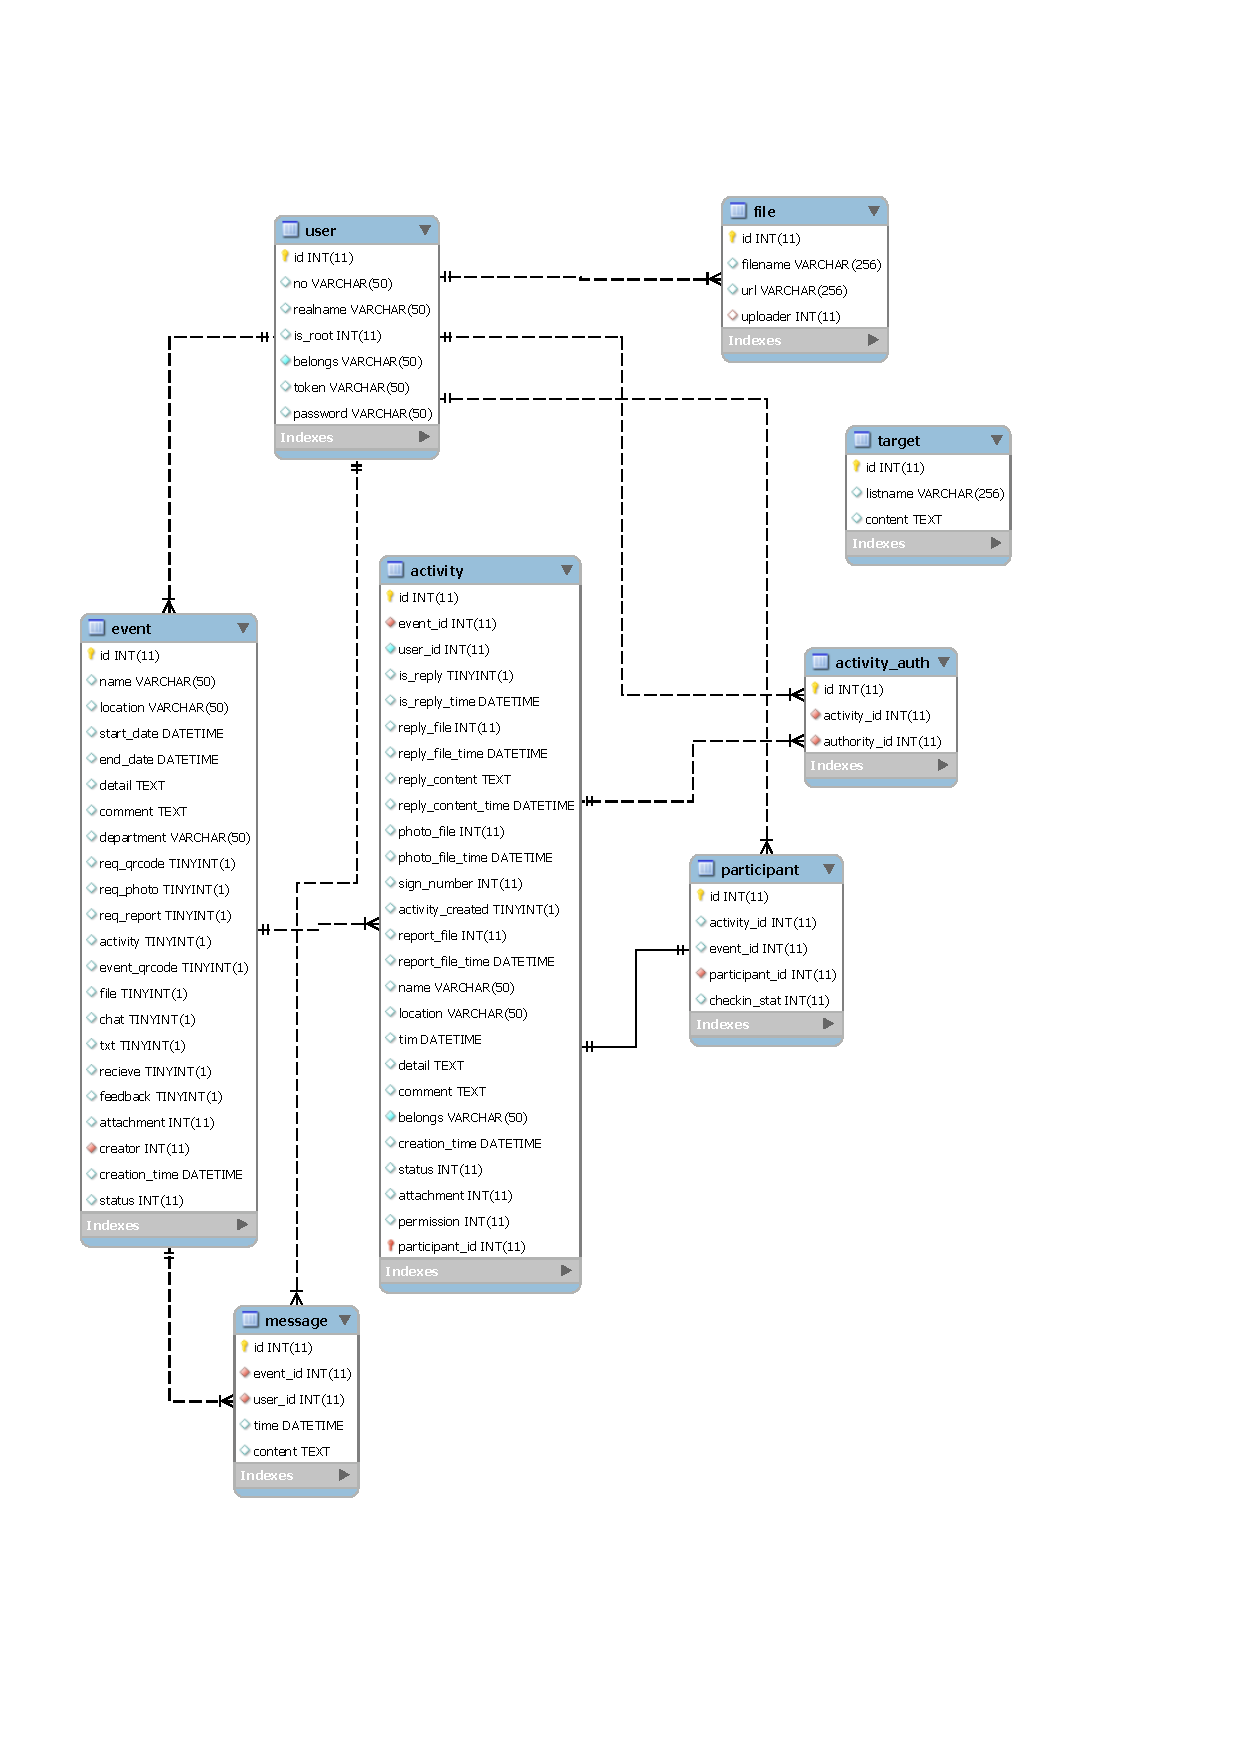
\includegraphics[width=0.8\textwidth]{uml}
  \caption{数据库UML图}
  \label{fig:uml}
\end{figure}

各个数据表的意义如下所述:

\begin{itemize}
\item user:用户数据表,存储了用户相关的信息;
\item file:上传的文件数据表,记录了文件在服务器上的路径、原始文件名以及文件的上传者ID;
\item event:活动数据表,记录了活动的详细信息;
\item activity:子活动数据表,记录了子活动的详细信息;
\item activity\_auth:子活动的授权人,通过两个外链通过一个用户ID和一个活动的ID连接了一个用户和一个活动,表示这个用户是这个活动的授权人之一;
\item message:用户对活动的反馈信息记录表,记录了一个反馈信息所属的活动、用户以及上传时间和反馈内容;
\item participant:记录了一个用户对子活动的参与情况,每一条记录表示了一个用户参与了一个特定的子活动;
\item target: 记录了来自Excel表的发送对象表,通过一个JSON Array保存了一个特定的用户群组。
\end{itemize}

通过对数据库的结构进行设计,可以使得每个API的调用都只会用到一句SQL语句就可以完成所需要的操作,保证了后端运行的效率和反应时间,提高了系统抗压能力,更能够提升用户的体验。

\section{功能详解}

通过\ref{requireAnalysis}节对需求的分析,结合对图\ref{fig:demand2}的分析,我们已经明确了各个角色所需要的功能,接下来需要对系统的具体功能进行设计。

一级管理者拥有对系统最高的控制权,可以指定新的管理员,也可以对分工会主席名单(发送范围)进行修改,并且可以创建只有一级管理者才能创建的活动。对于一级管理者来说,需要使用到的功能如图\ref{fig:level1}所示。

\begin{figure}[H]
  \centering
  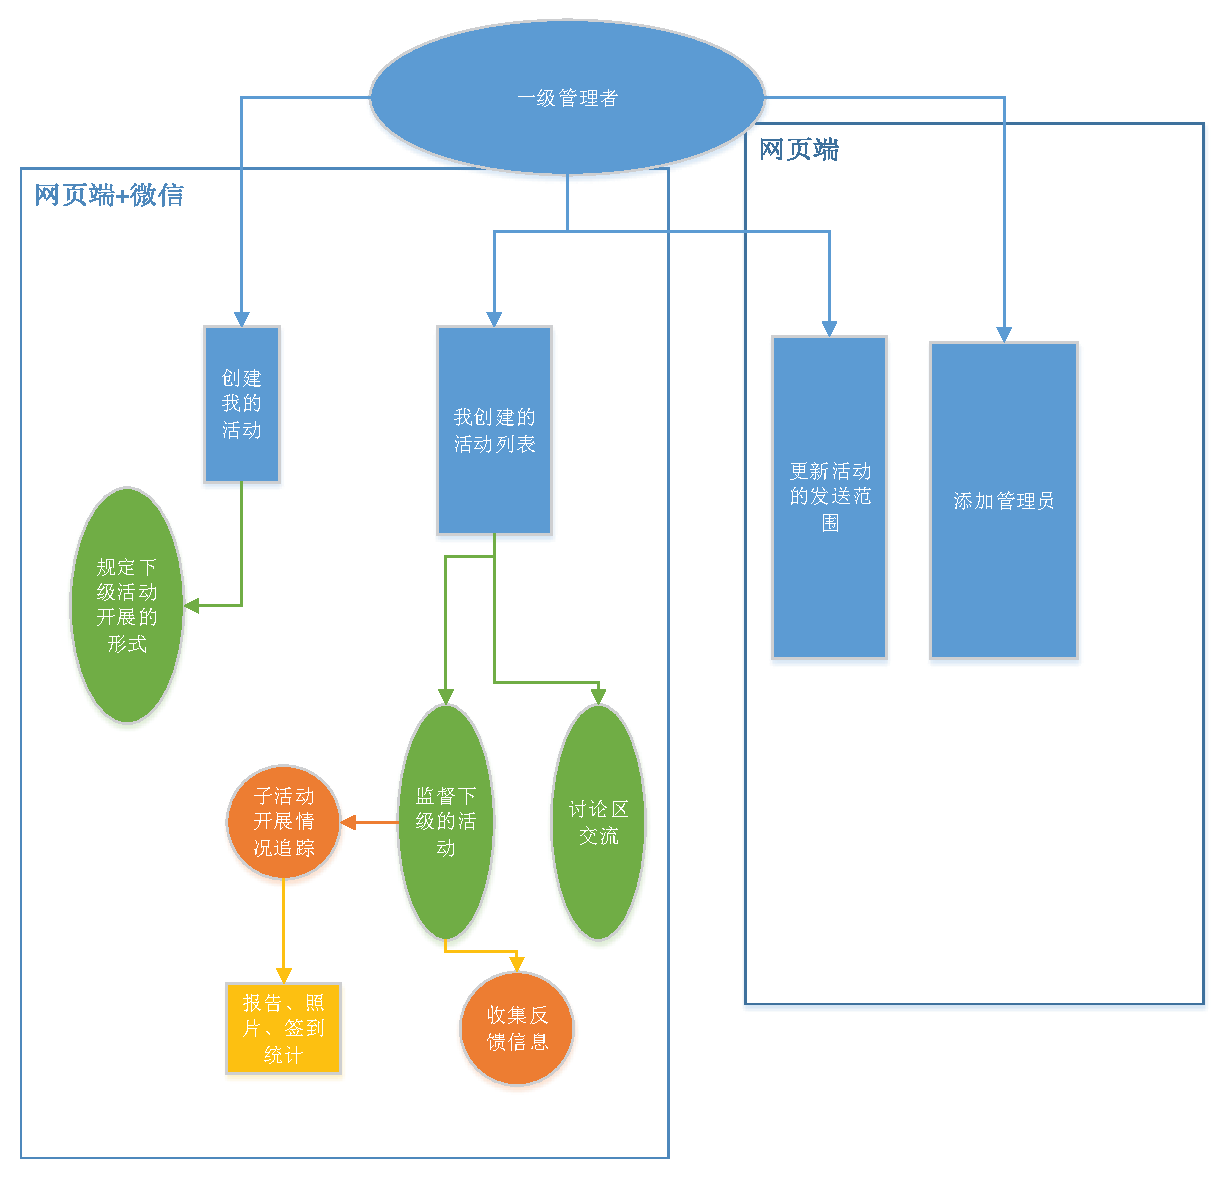
\includegraphics[width=1\textwidth]{level1}
  \caption{一级管理者的功能图}
  \label{fig:level1}
\end{figure}

当一级管理者创建一个活动并将这个活动的消息发送给一些分工会的主席的时候,这些分工会的主席便成为了二级授权者的角色。同时一级管理者可以将自己作为发送范围中的一员,使得自己成为某个活动的二级授权者,从而创建一个活动的子活动。

二级授权者可以将创建子活动的权利授权给另一个用户,使其代自己成为另一个该活动的二级授权者。一个二级授权者可以创建子活动,并对这个子活动进行全权操作。二级授权者的功能图如图\ref{fig:level2}所示。

\begin{figure}[H]
  \centering
  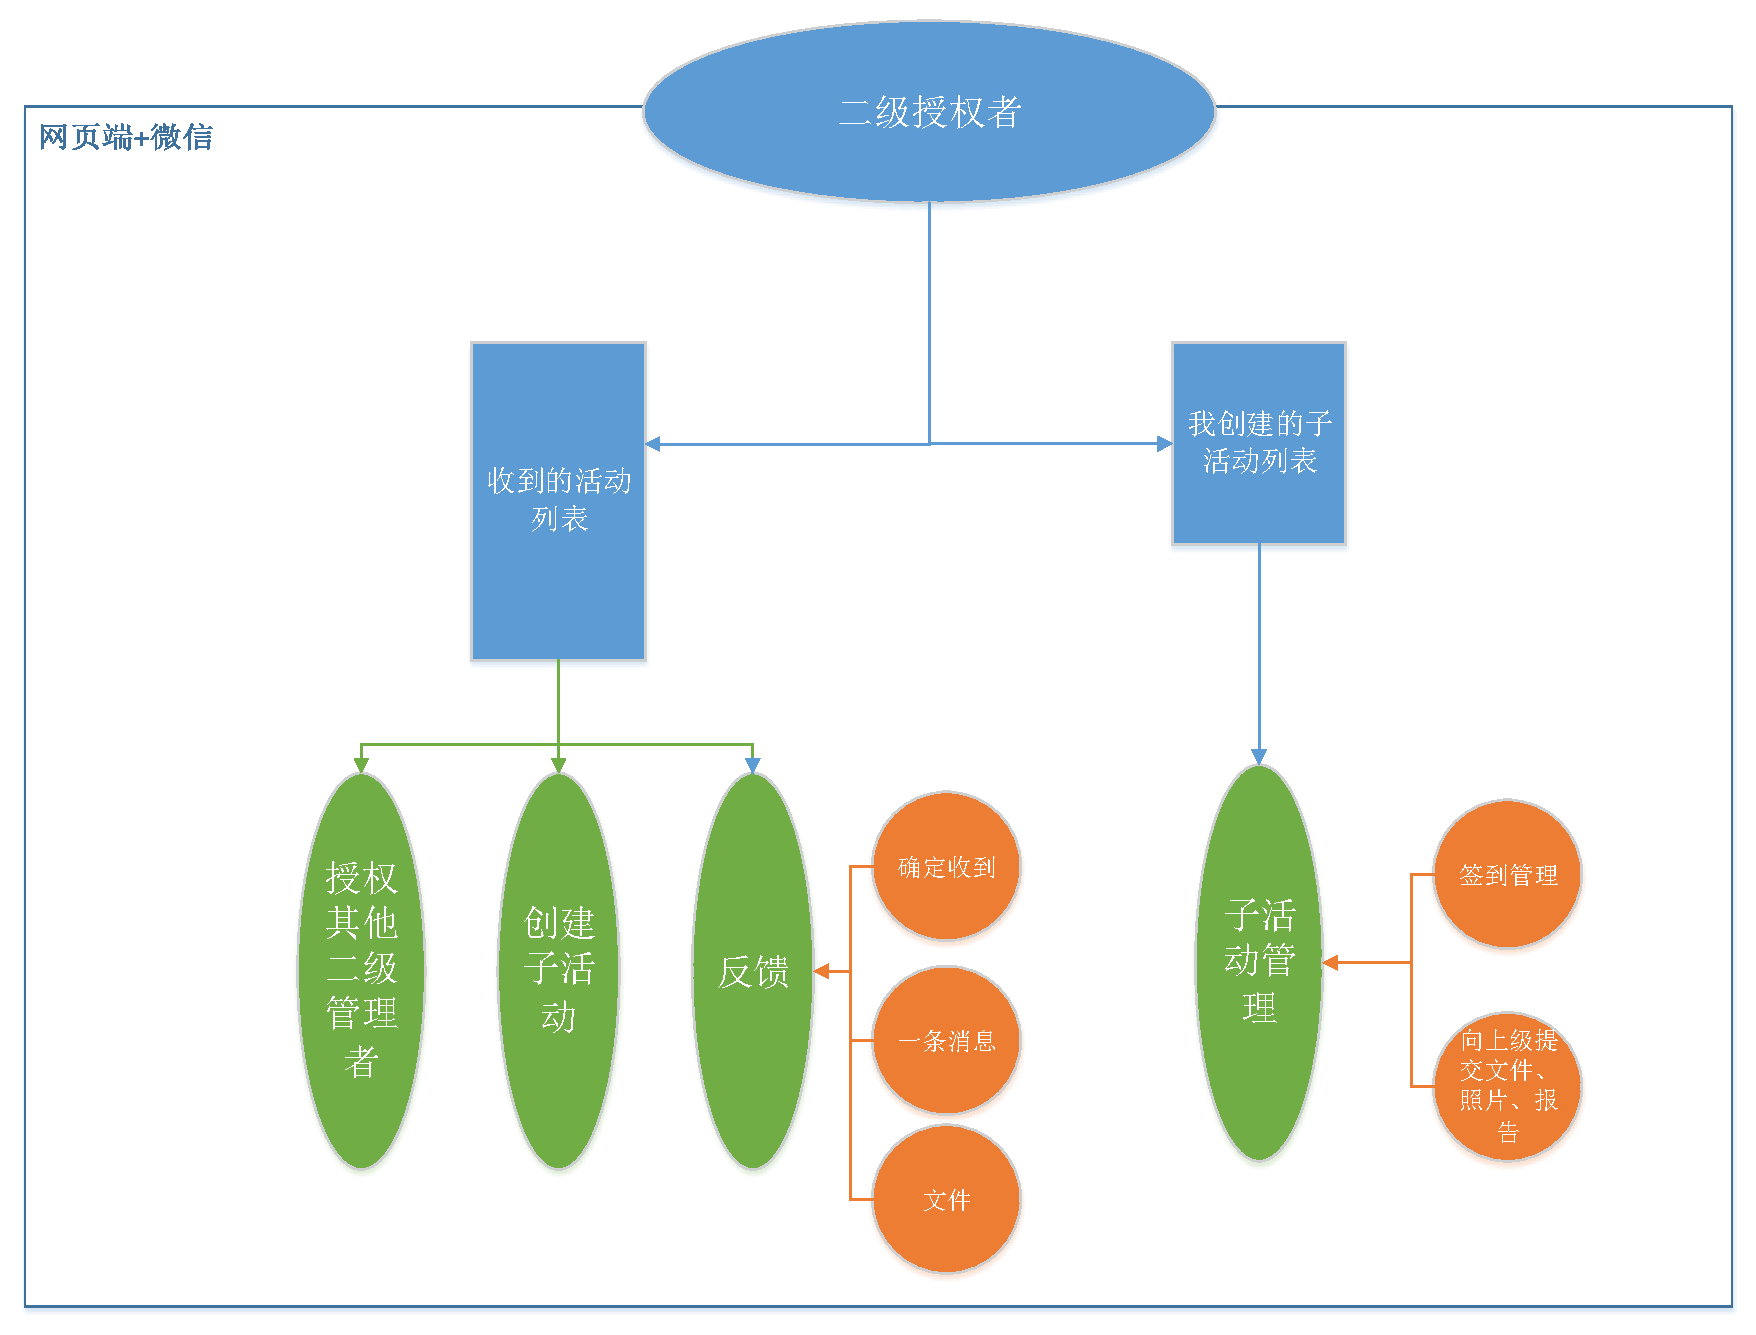
\includegraphics[width=1\textwidth]{level2}
  \caption{二级授权者的功能图}
  \label{fig:level2}
\end{figure}

三级接收者会在二级授权者创建子活动之后,在微信工会公众平台上收到活动信息推送,并选择子活动参与,通过签到确认活动的参与情况。同样的,二级授权者可以参与自己创建的子活动,并成为三级接收者的角色。

三级接收者的权限则十分受限,只能对接收活动和子活动的通知,并通过签到来确认参加活动。三级接收者的功能图如图\ref{fig:level3}所示。

\begin{figure}[H]
  \centering
  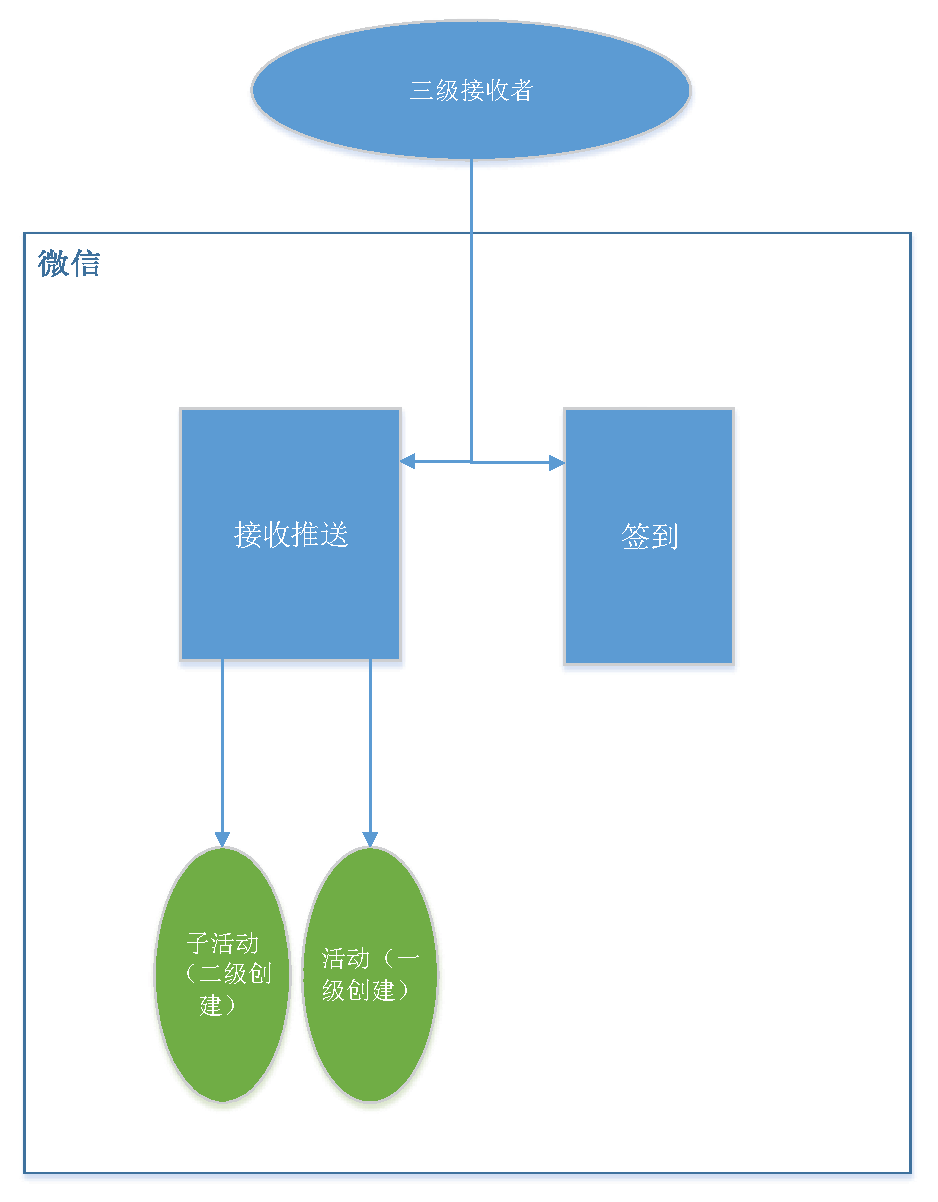
\includegraphics[width=0.6\textwidth]{level3}
  \caption{三级接收者的功能图}
  \label{fig:level3}
\end{figure}

为了完成这些功能,后端需要实现的API如表\ref{table:api}所示。表中给出了系统中用到的全部的API的介绍,以及能够调用该API的用户需要的权限。

\begin{table}[htb]
  \centering
  \caption{后端API表及调用权限}
  \label{table:api}
    \begin{tabular}{llccc}
      \toprule
      API & 描述 & 一级 & 二级 & 三级 \\
      \midrule % $\surd$
      AddActivityAuth 		& 添加一个授权人 			& 	& $\surd$	& \\
      AddParticipant 		& 参与一个子活动 			& 	&  	& $\surd$\\
      CreateActivity 		& 创建一个子活动 			& 	& $\surd$ 	& \\
      EndActivity 			& 结束一个子活动 			& $\surd$	& $\surd$ 	& \\
      GetActivityByEvent 	& 通过活动搜索子活动		& $\surd$	& $\surd$ 	& $\surd$\\
      GetActivityWithEvent 	& 得到一个子活动的详细信息 	& $\surd$	& $\surd$ 	&$\surd$ \\
      GetCreatedActivity 	& 获得当前用户创建的子活动 	& 	& $\surd$ 	& \\
      RenoticeActivity 		& 重新发送活动提醒 			& $\surd$	&  	& \\
      ActivityCheckin 		& 对一个活动进行签到 		& $\surd$	&  	& \\
      GenerateExcel 		& 创建Excel表格报告 		& $\surd$	&  	& \\
      GetCheckedParticipant & 获得一个活动的参与者 		& $\surd$	&  	& \\
      ManualCheckin 		& 手动进行签到 				& 	&  $\surd$	& \\
      CreateEvent 			& 创建一个活动 				& $\surd$	&  	& \\
      GetEventStat 			& 获得一个活动的参与情况 	& $\surd$	&  	& \\
      GetListEvent 			& 获得创建的活动列表 		& $\surd$	&  	& \\
      GetRecvEvent 			& 获得收到的活动列表 		& 	& $\surd$ 	& \\
      GetSingleEvent 		& 获得一个活动的详细信息 	& $\surd$	& $\surd$ 	& \\
      ReplyEvent 			& 对一个活动进行反馈 		& 	&  $\surd$	& \\
      UpdateEvent 			& 更新一个活动内容 			& $\surd$	&  	& \\
      GetFile 				& 得到一个上传的文件详细信息& $\surd$	& $\surd$ 	& $\surd$\\
      UploadFile 		& 上传一个文件 					& $\surd$	& $\surd$ 	& $\surd$\\
      UploadXls 		& 上传一个表格 					& $\surd$	&  	& \\
      GetMessage 		& 得到一个活动的讨论区内容 		& $\surd$	& $\surd$ 	& \\
      NewMessage 		& 添加讨论区内容 				& $\surd$	&  $\surd$	& \\
      UpdateMessage 	& 更新讨论区讨论内容 			& $\surd$	& $\surd$ 	& \\
      DelPostTarget 	& 删除一个用户群组 				& $\surd$	&  	& \\
      GetPostTarget 	& 得到一个用户群组中的用户ID 	& $\surd$	&  	& \\
      NewPostTarget 	& 创建一个新的用户群组 			& $\surd$	&  	& \\
      ChangePassword 	& 修改一个用户的密码 			& $\surd$	& $\surd$ 	&$\surd$ \\
      GetCurrentUser 	& 获得当前用户 					& $\surd$	& $\surd$ 	& $\surd$\\
      GetUserPubKey 	& 为当前登录行为提供一个RSA公钥 & $\surd$	& $\surd$ 	& $\surd$\\
      Login 			& 进行登录行为 					& $\surd$	& $\surd$ 	& $\surd$\\
      Logout 			& 用户登出 						& $\surd$	& $\surd$ 	& $\surd$\\
      SearchUser 		& 查找一个用户 					& $\surd$	&  	& \\
      SetRoot 			& 将一个用户设置为管理员 		& $\surd$	&  	& \\
      SignIn 			& 注册一个新用户 				& $\surd$	& $\surd$ 	&$\surd$ \\
      \bottomrule
    \end{tabular}
\end{table}

实现了这些功能之后,配合前端的界面呈现,系统就能够在各个平台为用户进行服务了。
